%!TEX TS-program = pdflatex
%!TEX root = tesi.tex
%!TEX encoding = UTF-8 Unicode

\chapter{Compression techniques for time series data}
Before venturing into modern time series compression algorithms, it is useful to have a brief
introduction into the basic techniques that can be used to achieve compression. In this chapter,
we will discuss the principles of delta-encoding, variable-length encoding, run-length encoding,
dictionary-based compression.

\section{Delta encoding}
Delta encoding is a technique in which the difference between sequential data is stored instead
of raw values. For example, suppose we have the following values:
$$V= 60, 61, 62, 60, 65$$
We can transform the values as differences plus the initial reference value:
$$V’= 60, 1, 1, -3, 5$$
Delta of delta encoding is a variation of delta encoding whereby we first transform a sequence
with deltas and we then re-apply the delta encoding. This can be achieved with the following
formula: $D = (t_{n} - t_{n-1}) - (t_{n-1} - t_{n-2})$, where $t$ is a value in the time series
sequence. This variation is useful when the deltas between values are big but almost always
the same, for example, if we record data every minute the delta between the timestamps measured
in seconds will always be 60, and by re-applying delta encoding we will transform the values
to 0. As an example, in the first column of Table~\ref{tab:delta}, we have 6 Unix time timestamps
in seconds. In the second column, we have the delta between these timestamps, while in the
third column we have the delta of delta.
Since the timestamps were collected roughly every minute, the delta is always around 60 seconds,
while the delta of the delta is always around 0. By storing the delta of deltas together with
an appropriate variable length code (described in the following section), one can reduce the
amount of storage needed as compared to storing the timestamps.
This technique is used in Gorilla \cite{Pelkonen:2015}, a time series database created
by Facebook to monitor their infrastructure, which we will analyze in chapter 3.

\begin{table}[]
\centering
\begin{tabular}{l|l|l}
\textbf{Timestamp}  & \textbf{Delta} & \textbf{Delta of Delta} \\ \hline
1567330058 & -     & -              \\
1567330118 & 60    & -              \\
1567330177 & 59    & -1             \\
1567330238 & 61    & 2              \\
1567330298 & 60    & 1              \\
1567330358 & 60    & 0              \\
\end{tabular}
\caption{A comparison between delta and delta of delta compression.}
\label{tab:delta}
\end{table}

\section{Variable-length encoding}
Variable-length encoding refers to the technique whereby, given a dataset made up of symbols
drawn by an alphabet, we replace symbols that occur more often with short codes and symbols
that occur less frequently with longer codes. The result is a long string of bits with no
separators between the codes of consecutive symbols. The decoder should be able to read this
string unambiguously into individual codes. Such codes are called "prefix codes"  in
Information Theory.
One example of a prefix code is Elias’ Gamma Code \cite{elias1975universal}. This code, designed for positive
integers, prefix each integer with a representation of its order of magnitude. Given a
positive integer $n$, proceed as follows:
\begin{itemize}
	\item Denote by $M$ the length of the binary representation of $n$.
	\item Prepend $M-1$ zeroes to $n$.
\end{itemize}\par
Table~\ref{tab:elias} shows some sample numbers encoded using the gamma code.
\begin{table}[]
\centering
\begin{tabular}{l|l}
\textbf{Number}     & \textbf{Gamma Encoded Number} \\ 
\hline
1          & 1                    \\ 
8          & 0001000              \\ 
12         & 0001100              \\ 
18         & 000010010            \\ 
\end{tabular}
\caption{Example of some Gamma encoded numbers.}
\label{tab:elias}
\end{table}
How can variable-length encoding help when dealing with time series data?
In many time series applications, the values we record are strongly correlated.
For example, if we are recording the temperature of a certain location every minute,
chances are that the value we record in a given minute is similar to its predecessor.
To exploit this fact, we may use delta encoding to store only the differences between each
value, and encode such value with a variable length code for integers, for example, the
Rice code \cite{Rice1979Some}. As a practical example, let us consider the following values:
$$V= 80, 82, 83, 81, 81$$
To compress these values, we first need to apply delta encoding:
$$V = 80, 2, 1, -2, 0$$
Now it is time to apply the Rice code. The Rice code depends on the choice of a base
$k$ and is computed in three steps. Given an integer number $n$, whose k-base representation
we call $N$, proceed as follows:
\begin{itemize}
	\item Separate the sign bit of $N$ from the rest of the number
	\item Separate the $k$ least significant bits of $N$. They become the least significant
    bits of the rice code
	\item Code the $j = \lfloor\frac{|n|}{2^k}\rfloor$ remaining bits as $j$ 1’s followed by a 0
	\item If $n$ is non-negative, prepend 0, else prepend 1
\end{itemize}
By applying these rules with $k = 2$, we obtain the codes in Table~\ref{tab:rice}
\begin{table}[]
\centering
\begin{tabular}{l|l}
\textbf{Initial number}     & \textbf{Number after compression} \\ 
\hline
80          & $0|111111111111111111110|00$ \\                    
82          & $0|0|10$                     \\ 
1           & $0|0|01$                     \\              
-2          & $1|0|10$                     \\           
0           & $0|0|00$                     \\            
\end{tabular}
\caption{On the first column, the original time series values.
On the second column, the binary representation of these numbers after applying delta and rice
encoding.}
\label{tab:rice}
\end{table}
We can store the whole sequence in 40 bits, which is a great improvement over storing each
value as a 32-bit integer. Most audio compression algorithms adopt this technique \cite{WikipediaContributors2019Golomb}.

\section{Run-lenght encoding}
For certain types of data adjacent symbols are often correlated, and there may be runs of an
identical symbol repeated that could be exploited for compression purposes. In general, the way
this is exploited is by replacing a long run with a pair (length, symbol). For example,
$(1, 10), (0, 5), (1, 10)$ is the short form the following sequence of values:
1, 1, 1, 1, 1, 1, 1, 1, 1, 1, 0, 0, 0, 0, 0, 1, 1, 1, 1, 1, 1, 1, 1, 1, 1.
In many applications where changes in data are rare this leads to good compression ratios;
on the contrary, if the data changes frequently using RLE results in expansion. In the
following chapter, we will talk about Sprintz \cite{blalock2018sprintz},
an algorithm designed to compress sensor-generated time series data, which uses, among other
techniques, run-length encoding.

\subsection*{Dictionary-based compression}
In text data, we can observe that words are often repeated. We can exploit this fact by
building a dictionary of words we encounter in a text and storing a reference to a dictionary
entry instead of storing the words again. The same idea can be extended to non-text data, for
example, we consider a sequence of numbers as an entry in our dictionary. Every time the
sequence is repeated, we can store a reference to it.
The entire field of dictionary-based compression was initiated with the algorithm published
in a seminal paper by Ziv and Lempel in 1977, commonly referred to as LZ77 \cite{ziv1977universal}.
LZ77 is based on the concept of a sliding window. The window is divided into a search buffer
and a look-ahead buffer. The search buffer contains the dictionary and the data that has been
recently processed. The input that has not been read and encoded yet resides in the look-ahead
buffer.
The algorithm can be described as follows. Let $S[0...j -1]$ be the search buffer, 
$L[0...k-1]$ be the look-ahead buffer (starting at position $j$) and $W(0...j+k-1)$
be the entire window. Let $C(x)$ denote the default code for symbol $x$.
Every symbol will be represented by a pointer structured like the following
$<off, len, C(x)>$, where $off$ is the distance from the current symbol to the
position in the search buffer and $len$ is the length of the matched string.
\begin{enumerate}
	\item let $w[p...q]$, $p < j$ be the longest string that has a match beginning at $L[0]$

	\item if no match encode $<0, 0, C(L[0])>$

	\item else encode $<p, q - p + 1, C(L[q - p + 1])$

	\item advance search and look-ahead buffers by $len + 1$ symbols, where $len$ is the length
    of the matched string
\end{enumerate}
As a practical example, let us try to encode the following sequence:
\begin{center}
Seq = c a b r a c a d a b r a r r a r r a d
\end{center}
For this example we will use $j=7$ and $k=6$. The sequence encoding is described in Table~\ref{tab:lz}.
\begin{table}[!htbp]
\centering
\begin{tabular}{p{1.5cm}|p{2.5cm}|p{3.5cm}|p{2cm}}
\textbf{Search buffer} & \textbf{Look-ahead buffer} & \textbf{Longest string} \newline \textbf{matching} $L[0...k]$ \newline \textbf{for some} $k$ & \textbf{Encoded symbol} \\
\hline
cabrace          & dabrar & /     & $<0, 0, d>$ \\                
abracad          & abrarr & abra  & $<0, 4, r>$ \\ 
adabrar          & rarrad & rarra & $<4, 5, d>$ \\               
\end{tabular}
\caption{Example of dictionary-based encoding using a sliding window.}
\label{tab:lz}
\end{table}

The encoded sequence will look like this: cabraca$<0,0,d><0, 4, r><4, 5, d>$.
Over the years, many different variations of this algorithm have been proposed,
but the basic principles are to be found in every general-purpose compression algorithm.

\section{Huffman encoding}
Huffman encoding is a lossless compression algorithm that produces a variable-length code,
whereby each symbol is associated with a given prefix which length is proportional
to the number of occurrences of the symbol. The algorithm uses a binary tree of nodes.
Each node can be a leaf node or an internal node and contains a value (a character) and a
frequency. To build up the tree, apply the following steps:
\begin{enumerate}
    \item create a leaf node for each character and add them to a priority queue, where
    the priority is the inverse of the frequency in which they occur
    \item while there is more than one node in the queue
    \begin{enumerate}
        \item remove the two nodes of highest priority (lowest frequency from the queue)
        \item add a new internal node with the two nodes as children and with a frequency
        equals to the sum of the frequency of the two nodes. Add this node to the priority queue
    \end{enumerate}
    \item the remaining node is the root node and the tree is complete
\end{enumerate}
The leaf of the tree contains all the characters we wanted to encode. The build the prefix
code for a given character, we traverse the tree until the node containing the character is
found. Every left turn is encoded as 0 while the right turn is encoded as 1.
As a practical example, consider the characters A, B, C, D with the associated frequency
3, 5, 7, 2. After having executed step 1, we are entering the loop of step 2.
We remove the node A and D since they have the lowest frequency and we add a new node
(let us call it E) to the tree with frequency 5 having A as a left child and D as a right
child. We also add this node to the priority queue. The next nodes to be removed from the
priority queue are B and E. We create a new node F, with frequency 10, that has B as a left
child and E as a right child. We add F to the priority queue.
We have two nodes left in the priority queue, C and F. We remove them, and we create a new
node G, with frequency 17 that has C as a left child and F as right child. We then add this
node to the priority queue. At this point, the loop ends as our tree is already completed.
The resulting tree is depicted in Figure~\ref{huffman_tree}.

\begin{figure}[!htbp]
\begin{center}
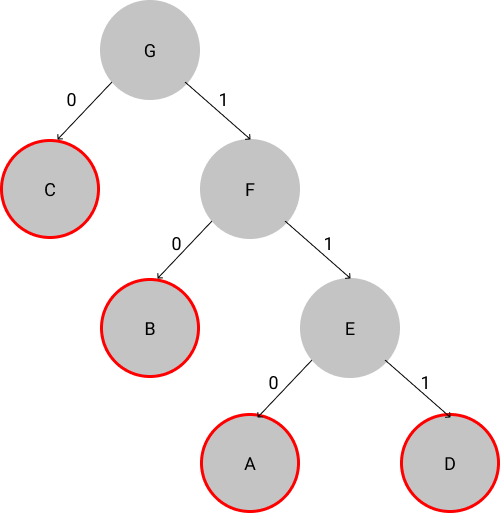
\includegraphics[width=200pt]{huffmanTree}
\caption[huffman_tree]{Huffman tree for characters A, B, C, D with frequency 3, 5, 7, 2.}
\label{huffman_tree}
\end{center}
\end{figure}